\PassOptionsToPackage{unicode=true}{hyperref} % options for packages loaded elsewhere
\PassOptionsToPackage{hyphens}{url}
%
\documentclass[10pt,xcolor=table,color={dvipsnames,usenames},ignorenonframetext,usepdftitle=false,french]{beamer}
\setbeamertemplate{caption}[numbered]
\setbeamertemplate{caption label separator}{: }
\setbeamercolor{caption name}{fg=normal text.fg}
\beamertemplatenavigationsymbolsempty
\usepackage{caption}
\captionsetup{skip=0pt,belowskip=0pt}
%\setlength\abovecaptionskip{-15pt}
\usepackage{lmodern}
\usepackage{amssymb,amsmath,mathtools,multirow}
\usepackage{float,hhline}
\usepackage{tikz}
\usepackage[tikz]{bclogo}
\usepackage{mathtools}
\usepackage{ifxetex,ifluatex}
\usepackage{fixltx2e} % provides \textsubscript
\ifnum 0\ifxetex 1\fi\ifluatex 1\fi=0 % if pdftex
  \usepackage[T1]{fontenc}
  \usepackage[utf8]{inputenc}
  \usepackage{textcomp} % provides euro and other symbols
\else % if luatex or xelatex
  \usepackage{unicode-math}
  \defaultfontfeatures{Ligatures=TeX,Scale=MatchLowercase}
\fi
\usetheme[coding=utf8,language=french,
,titlepagelogo=img/LOGO-ENSAE.png
]{TorinoTh}
% use upquote if available, for straight quotes in verbatim environments
\IfFileExists{upquote.sty}{\usepackage{upquote}}{}
% use microtype if available
\IfFileExists{microtype.sty}{%
\usepackage[]{microtype}
\UseMicrotypeSet[protrusion]{basicmath} % disable protrusion for tt fonts
}{}
\IfFileExists{parskip.sty}{%
\usepackage{parskip}
}{% else
\setlength{\parindent}{0pt}
\setlength{\parskip}{6pt plus 2pt minus 1pt}
}
\usepackage{hyperref}
\hypersetup{
            pdftitle={Word-Embedding et sentiments des ménages avec Twitter},
            pdfauthor={Kim Antunez, Romain Lesauvage et Alain Quartier-la-Tente},
            pdfborder={0 0 0},
            breaklinks=true}
\urlstyle{same}  % don't use monospace font for urls
\newif\ifbibliography
% Prevent slide breaks in the middle of a paragraph:
\widowpenalties 1 10000
\raggedbottom
\AtBeginPart{
  \let\insertpartnumber\relax
  \let\partname\relax
  \frame{\partpage}
}
\AtBeginSection{
  \ifbibliography
  \else
    \begin{frame}{Sommaire}
    \tableofcontents[currentsection, hideothersubsections]
    \end{frame}
  \fi
}
\setlength{\emergencystretch}{3em}  % prevent overfull lines
\providecommand{\tightlist}{%
  %\setlength{\itemsep}{0pt}
  \setlength{\parskip}{0pt}
  }
\setcounter{secnumdepth}{0}

% set default figure placement to htbp
\makeatletter
\def\fps@figure{htbp}
\makeatother

\usepackage{wrapfig}
\usepackage{booktabs}
\usepackage{longtable}
\usepackage{array}
\usepackage{multirow}
\usepackage{wrapfig}
\usepackage{float}
\usepackage{colortbl}
\usepackage{pdflscape}
\usepackage{tabu}
\PassOptionsToPackage{dvipsnames}{xcolor}
\usepackage{threeparttable}
\usepackage{threeparttablex}
\usepackage[normalem]{ulem}
\usepackage{makecell}
\usepackage{animate}
\usepackage{fontawesome5}
\usepackage{caption}
\usepackage{graphicx}
\usepackage{tikz}
\usetikzlibrary{decorations}
\usetikzlibrary{decorations.pathmorphing}
\usetikzlibrary{decorations.pathreplacing}
\usetikzlibrary{decorations.shapes}
\usetikzlibrary{decorations.text}
\usetikzlibrary{decorations.markings}
\usetikzlibrary{decorations.fractals}
\usetikzlibrary{decorations.footprints}
\usepackage{hyperref}
\usepackage[T1]{fontenc}
\usepackage[utf8]{inputenc}
\usepackage{lmodern}
\usepackage{babel}
\usepackage{cancel}
\usepackage{array}

\title{\emph{Word-Embedding} et sentiments des ménages avec Twitter}
\ateneo{Projet de statistique appliquée, Ensae}
\author{Kim Antunez, Romain Lesauvage et Alain Quartier-la-Tente}
\date{}


\setrellabel{}

\setcandidatelabel{}

\rel{}
\division{11/06/2020}

\departement{Ensae — 2019-2020}
\makeatletter
\let\@@magyar@captionfix\relax
\makeatother

\DeclareMathOperator{\Cov}{Cov}
\newcommand{\E}[1]{\mathbb{E}\left[ #1 \right]}
\newcommand{\V}[1]{\mathbb{V}\left[ #1 \right]}
\newcommand{\cov}[2]{\Cov\left( #1\,,\,#2 \right)}

\begin{document}
\begin{frame}[plain,noframenumbering]
\titlepage
\end{frame}

\hypertarget{introduction}{%
\section{Introduction}\label{introduction}}

\begin{frame}{Introduction}
\protect\hypertarget{introduction-1}{}

\end{frame}

\hypertarget{word2vec}{%
\section{\texorpdfstring{\emph{word2vec}}{word2vec}}\label{word2vec}}

\hypertarget{uxe9valuation-du-moduxe8le}{%
\section{Évaluation du modèle}\label{uxe9valuation-du-moduxe8le}}

\begin{frame}{Évaluation sur le corpus de tweets (1/2)}
\protect\hypertarget{uxe9valuation-sur-le-corpus-de-tweets-12}{}

\begin{figure}
\begin{minipage}{.4\textwidth}


« Notre » modèle

\medskip

\footnotesize
\textbf{ Spearman : } 0,57 (p-v : 4,1 \%)
\normalsize

\medskip

\faArrowCircleRight{} \textbf{bons} résultats


\end{minipage}%
\begin{minipage}{.6\textwidth}
\tiny

\begin{table}[!h]
\begin{center}
\begin{tabular}{|c|c|c|c|}
    \hline
\textbf{bonjour} & \textbf{femme} & \textbf{1} & \textbf{samedi} \tabularnewline
\emph{(669)} & \emph{(264)} & \emph{(765)} & \emph{(203)} \tabularnewline
       \hline

\includegraphics[height=2mm]{img/emojis/1.png} (0,59) & quelle (0,49) & 5 (0,55) & soir (0,57) \tabularnewline

\includegraphics[height=2mm]{img/emojis/2.png} (0,59) & cette (0,46) & mois (0,51) & vivement (0,51) \tabularnewline
merci (0,54) & une (0,44) & 10 (0,49) & demain (0,50) \tabularnewline
nuit (0,48) & vie (0,44) & 2 (0,48) & end (0,48) \tabularnewline
bisous (0,47) & grippe (0,44) & top (0,48) & weekend (0,47) \tabularnewline
bonne (0,47) & belle (0,43) & depuis (0,47) & matin (0,45) \tabularnewline

\includegraphics[height=2mm]{img/emojis/3.png} (0,46) & ma (0,43) & saison (0,46) & jeudi (0,45) \tabularnewline
vous (0,46) & magnifique (0,43) & ans (0,44) & prochain (0,43) \tabularnewline
plaisir (0,44) & nouvelle (0,43) & jours (0,43) & week (0,43) \tabularnewline
allez (0,43) & vidéo (0,39) & 3 (0,43) & 
\includegraphics[height=2mm]{img/emojis/4.png} (0,42) \tabularnewline
    \hline
 \end{tabular}
\captionsetup{margin=0cm,format=hang,justification=justified}

\end{center}
\emph{ep = 80 / w = 4 / lr = 0,02 / dim = 100 / base : 100 000 tweets}

\end{table}
\normalsize


\end{minipage}
\end{figure}

\pause

\begin{figure}
\begin{minipage}{.4\textwidth}

Modèle \texttt{Gensim}

\medskip

\footnotesize
\textbf{ Spearman : } 0,50 (p-v : 0,0 \%)
\normalsize

\medskip

\faArrowCircleRight{} \textbf{très bons} résultats

\end{minipage}%
\begin{minipage}{.6\textwidth}
\tiny

\begin{table}[h]
\begin{center}
\begin{tabular}{|c|c|c|c|}
    \hline
\textbf{bonjour} & \textbf{femme} & \textbf{1} & \textbf{samedi} \tabularnewline
\emph{(17 043)} & \emph{(6 177)} & \emph{(21 055)} & \emph{(4 917)} \tabularnewline
       \hline
bonsoir (0,85) & fille (0,86) & 2 (0,65) & vendredi (0,88) \tabularnewline
bjr (0,75) & copine (0,74) & 3 (0,64) & jeudi (0,86) \tabularnewline
hello (0,71) & meuf (0,71) & 6 (0,63) & lundi (0,83) \tabularnewline
salut (0,66) & demoiselle (0,66) & 4 (0,62) & mercredi (0,83) \tabularnewline
coucou (0,55) & nana (0,66) & 7 (0,60) & dimanche (0,83) \tabularnewline
transmets (0,49) & nièce (0,66) & 5 (0,58) & mardi (0,76) \tabularnewline
désagrément (0,48) & sœur (0,65) & 9 (0,58) & demain (0,72) \tabularnewline
avezvous (0,48) & barbe (0,65) & 8 (0,56) & barathon (0,56) \tabularnewline
bettembourg (0,48) & maman (0,64) & 1e (0,55) & 22h45 (0,55) \tabularnewline
hey (0,47) & princesse (0,64) & 34 (0,53) & 20h (0,54) \tabularnewline
    \hline
 \end{tabular}
\captionsetup{margin=0cm,format=hang,justification=justified}
\end{center}
\emph{ep = 100 / w = 4 / lr = 0,02 / dim = 100 / base : ensemble des tweets}

\medskip

\footnotesize{10 plus proches voisins par similarité cosinus}
\end{table}

\normalsize

\end{minipage}
\end{figure}

\end{frame}

\begin{frame}{Évaluation sur le corpus de tweets (2/2)}
\protect\hypertarget{uxe9valuation-sur-le-corpus-de-tweets-22}{}

\begin{figure}
\begin{minipage}{.5\textwidth}

\begin{center}
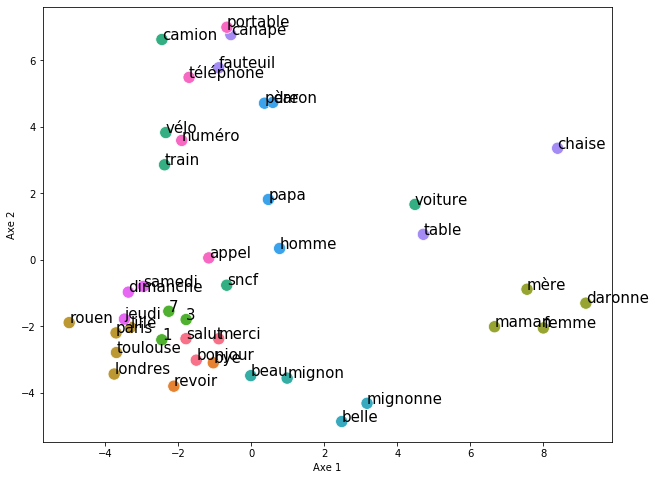
\includegraphics[width=0.95\textwidth]{img/acp_gensim.png}
\end{center}
\emph{ACP sur un corpus réduit de mots.}


\end{minipage}%
\begin{minipage}{.5\textwidth}

  \centering
  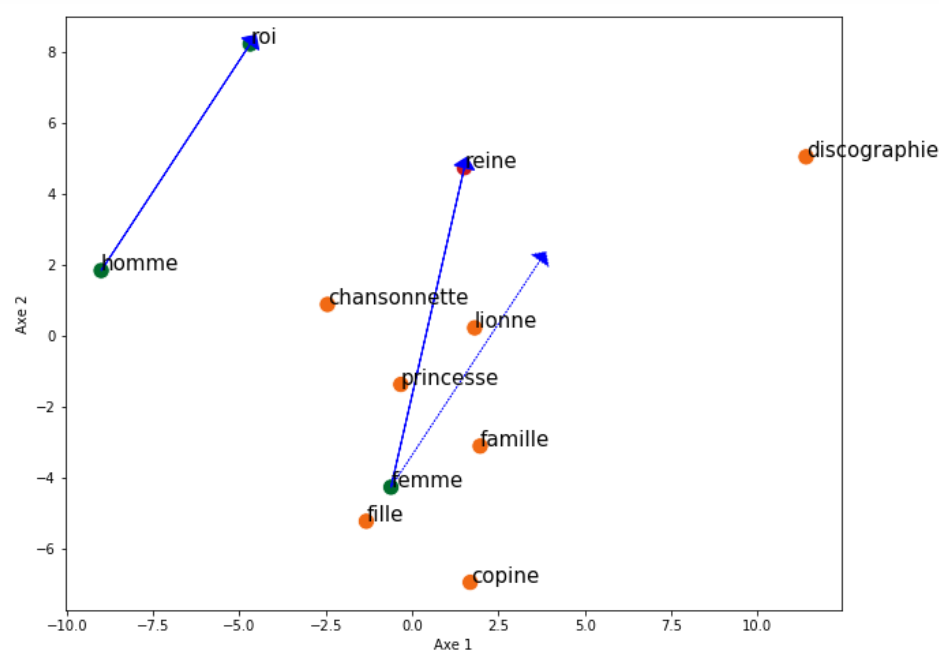
\includegraphics[width=\linewidth]{img/acp_reine.png}
  \emph{$\protect\overrightarrow{Roi} - \protect\overrightarrow{Homme} + \protect\overrightarrow{Femme} = $ ?}

\end{minipage}

\end{figure}

\medskip

\faArrowCircleRight{} Réduction de dimension des vecteurs-mots et
(parfois) opérations sur les mots \textbf{convaincants}

\end{frame}

\begin{frame}{Merci pour votre attention}
\protect\hypertarget{merci-pour-votre-attention}{}

\href{https://github.com/ARKEnsae/TweetEmbedding}{\faGithub{} ARKEnsae/TweetEmbedding}

\href{https://arkensae.github.io//TweetEmbedding/Redaction/Rapport_Final/Rapport.pdf}{\faEdit{} Rapport du projet}

\begin{center}

\includegraphics[width = 2.5cm]{img/LOGO-ENSAE.png}
\end{center}

\end{frame}

\end{document}
